\documentclass[a4paper,12pt]{article}

\usepackage[utf8]{inputenc}
\usepackage[T1]{fontenc}
\usepackage[english]{babel}
\usepackage{geometry}
\geometry{a4paper, margin=1in}
\usepackage{amsmath,amssymb}
\usepackage{booktabs,tabularx}
\usepackage{graphicx}
\usepackage{float}
\usepackage{hyperref}
\usepackage{enumitem}
\usepackage{longtable}
\usepackage{subcaption}

\title{Machine Learning Course Project Report\\Text Classification on AG News}
\author{
Tran Hoang Vy Khang (2352502)\\
Le Tan Minh Khoa (2352563)\\
Tao Nguyen Quang Khang (2352499)\\
Tran Gia Huy (2252264)\\
Vo Le Hai Dang (2352257)
}
\date{Semester I, 2025--2026}

\begin{document}

\maketitle

\section{Course Context}
\begin{itemize}[leftmargin=*]
    \item Course: Machine Learning (CO3117)
    \item Department: Computer Science and Engineering, HCMUT -- VNU-HCM
    \item Supervisor: Dr. Le Thanh Sach
    \item Topic: Text Data Classification (Topic 2)
\end{itemize}

\section{Project Objectives}
The project aims to build a complete text classification pipeline from exploratory data analysis to final model comparison, following the required workflow:
\begin{enumerate}[leftmargin=*]
    \item EDA and data understanding.
    \item Configurable preprocessing and TF-IDF feature extraction.
    \item Classical ML training and evaluation (Logistic Regression, SVM, Naive Bayes).
    \item Modern embedding extension with SBERT.
    \item Comparison across feature families with report-ready artifacts.
\end{enumerate}

\section{Dataset and Problem Setting}
\begin{itemize}[leftmargin=*]
    \item Dataset: \texttt{ag\_news} from Hugging Face Datasets.
    \item Task: 4-class news topic classification.
    \item Split used in full mode: 120,000 training samples and 7,600 test samples.
\end{itemize}

\section{Source Code and Reproducibility}
The complete source code, artifacts, and instructions to run this project are available on our public GitHub repository:
\begin{center}
    \url{https://github.com/THVKhang/MachineLearning_TextModule}
\end{center}
All executions are designed to be reproducible via a single Colab Notebook entry point, without requiring personal cloud storage mounting.

\section{Exploratory Data Analysis (EDA)}
Extensive Exploratory Data Analysis was performed to understand the characteristics of the AG News dataset. 

\begin{figure}[H]
    \centering
    \begin{subfigure}[b]{0.45\textwidth}
        \centering
        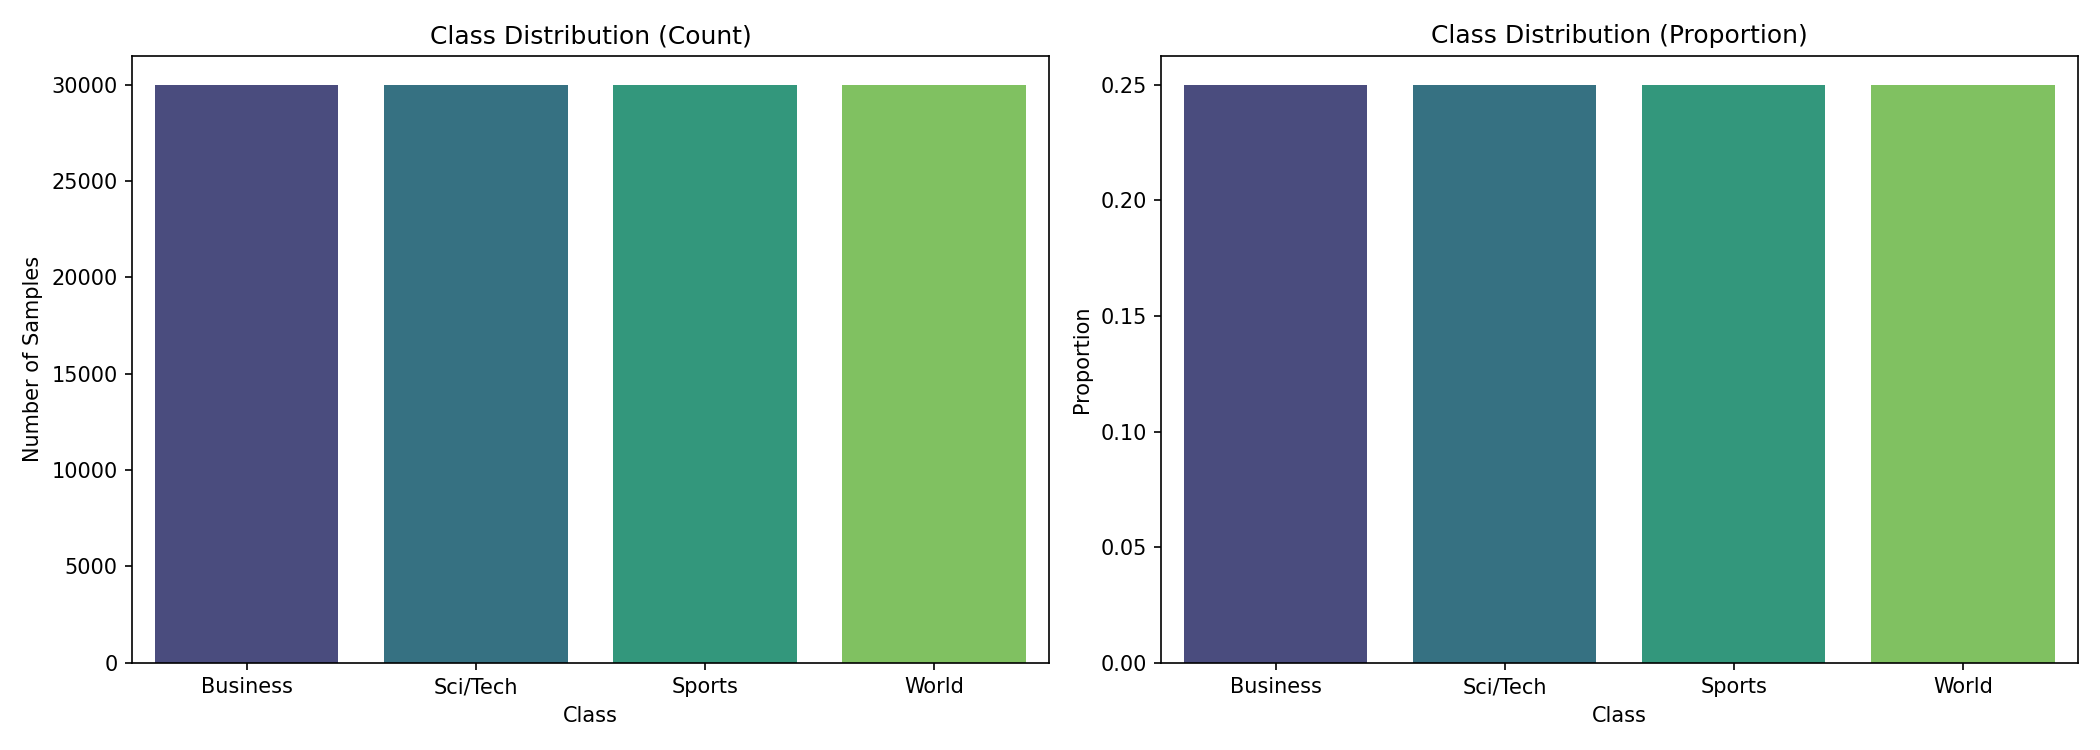
\includegraphics[width=\textwidth]{eda/class_distribution.png}
        \caption{Class Distribution}
    \end{subfigure}
    \hfill
    \begin{subfigure}[b]{0.45\textwidth}
        \centering
        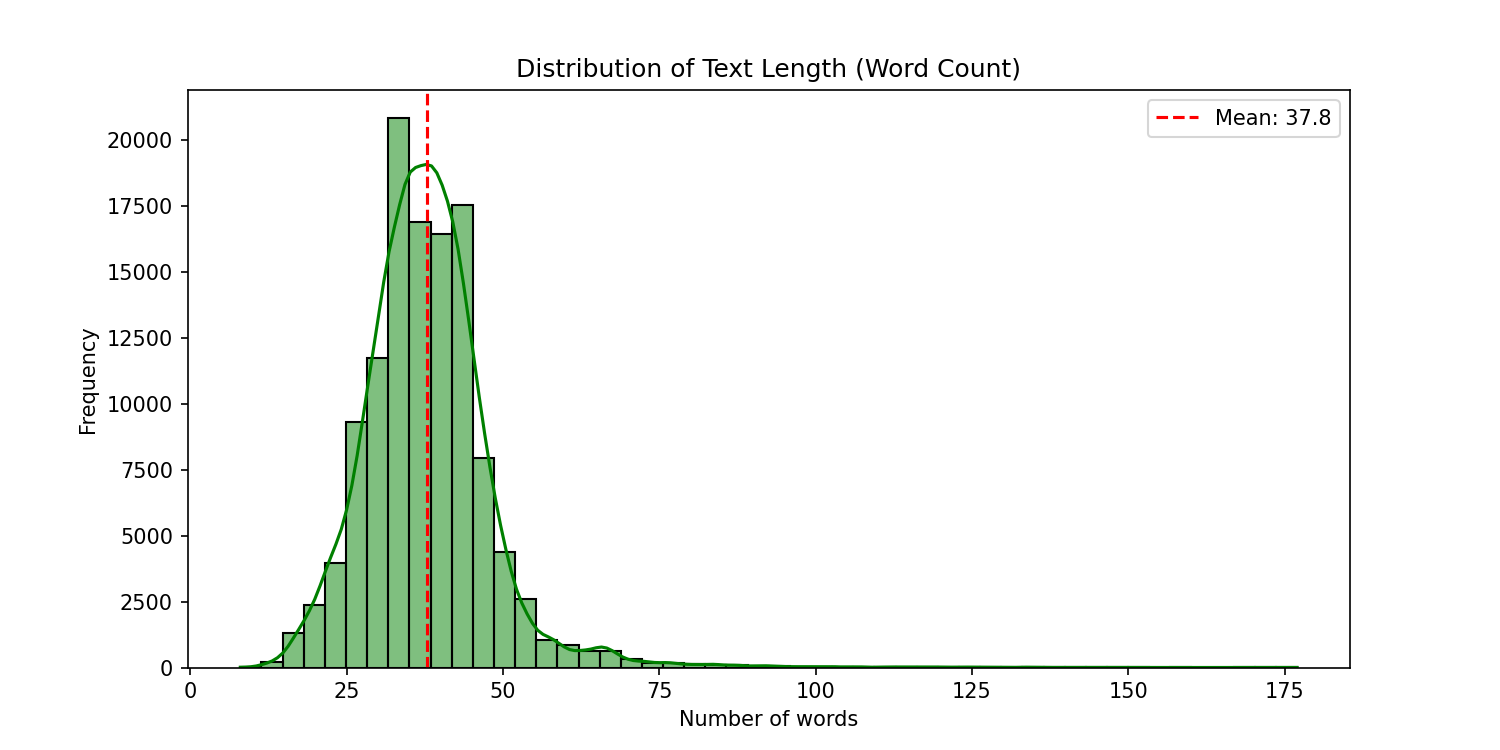
\includegraphics[width=\textwidth]{eda/text_length_distribution.png}
        \caption{Text Length Distribution}
    \end{subfigure}
    \caption{Overview of Dataset Distributions}
\end{figure}

Key findings include:
\begin{itemize}[leftmargin=*]
    \item \textbf{Balanced dataset:} The 120,000 training samples are perfectly balanced across the 4 classes (~30,000 each). This eliminates the need for class weighting or resampling techniques.
    \item \textbf{Short texts:} The average text length is approximately 35 words. Most semantic content can be captured effectively using TF-IDF with bigrams.
    \item \textbf{Domain-specific vocabulary:} Each class has distinct top keywords (e.g., `game'' for Sports, `stock'' for Business).
    \item \textbf{Low noise:} The dataset is very clean, with near-zero empty or duplicate texts.
    \item \textbf{Minimal URLs:} Only about 32 URL-heavy texts were found in the training set, having negligible impact on overall quality.
\end{itemize}

\begin{figure}[H]
    \centering
    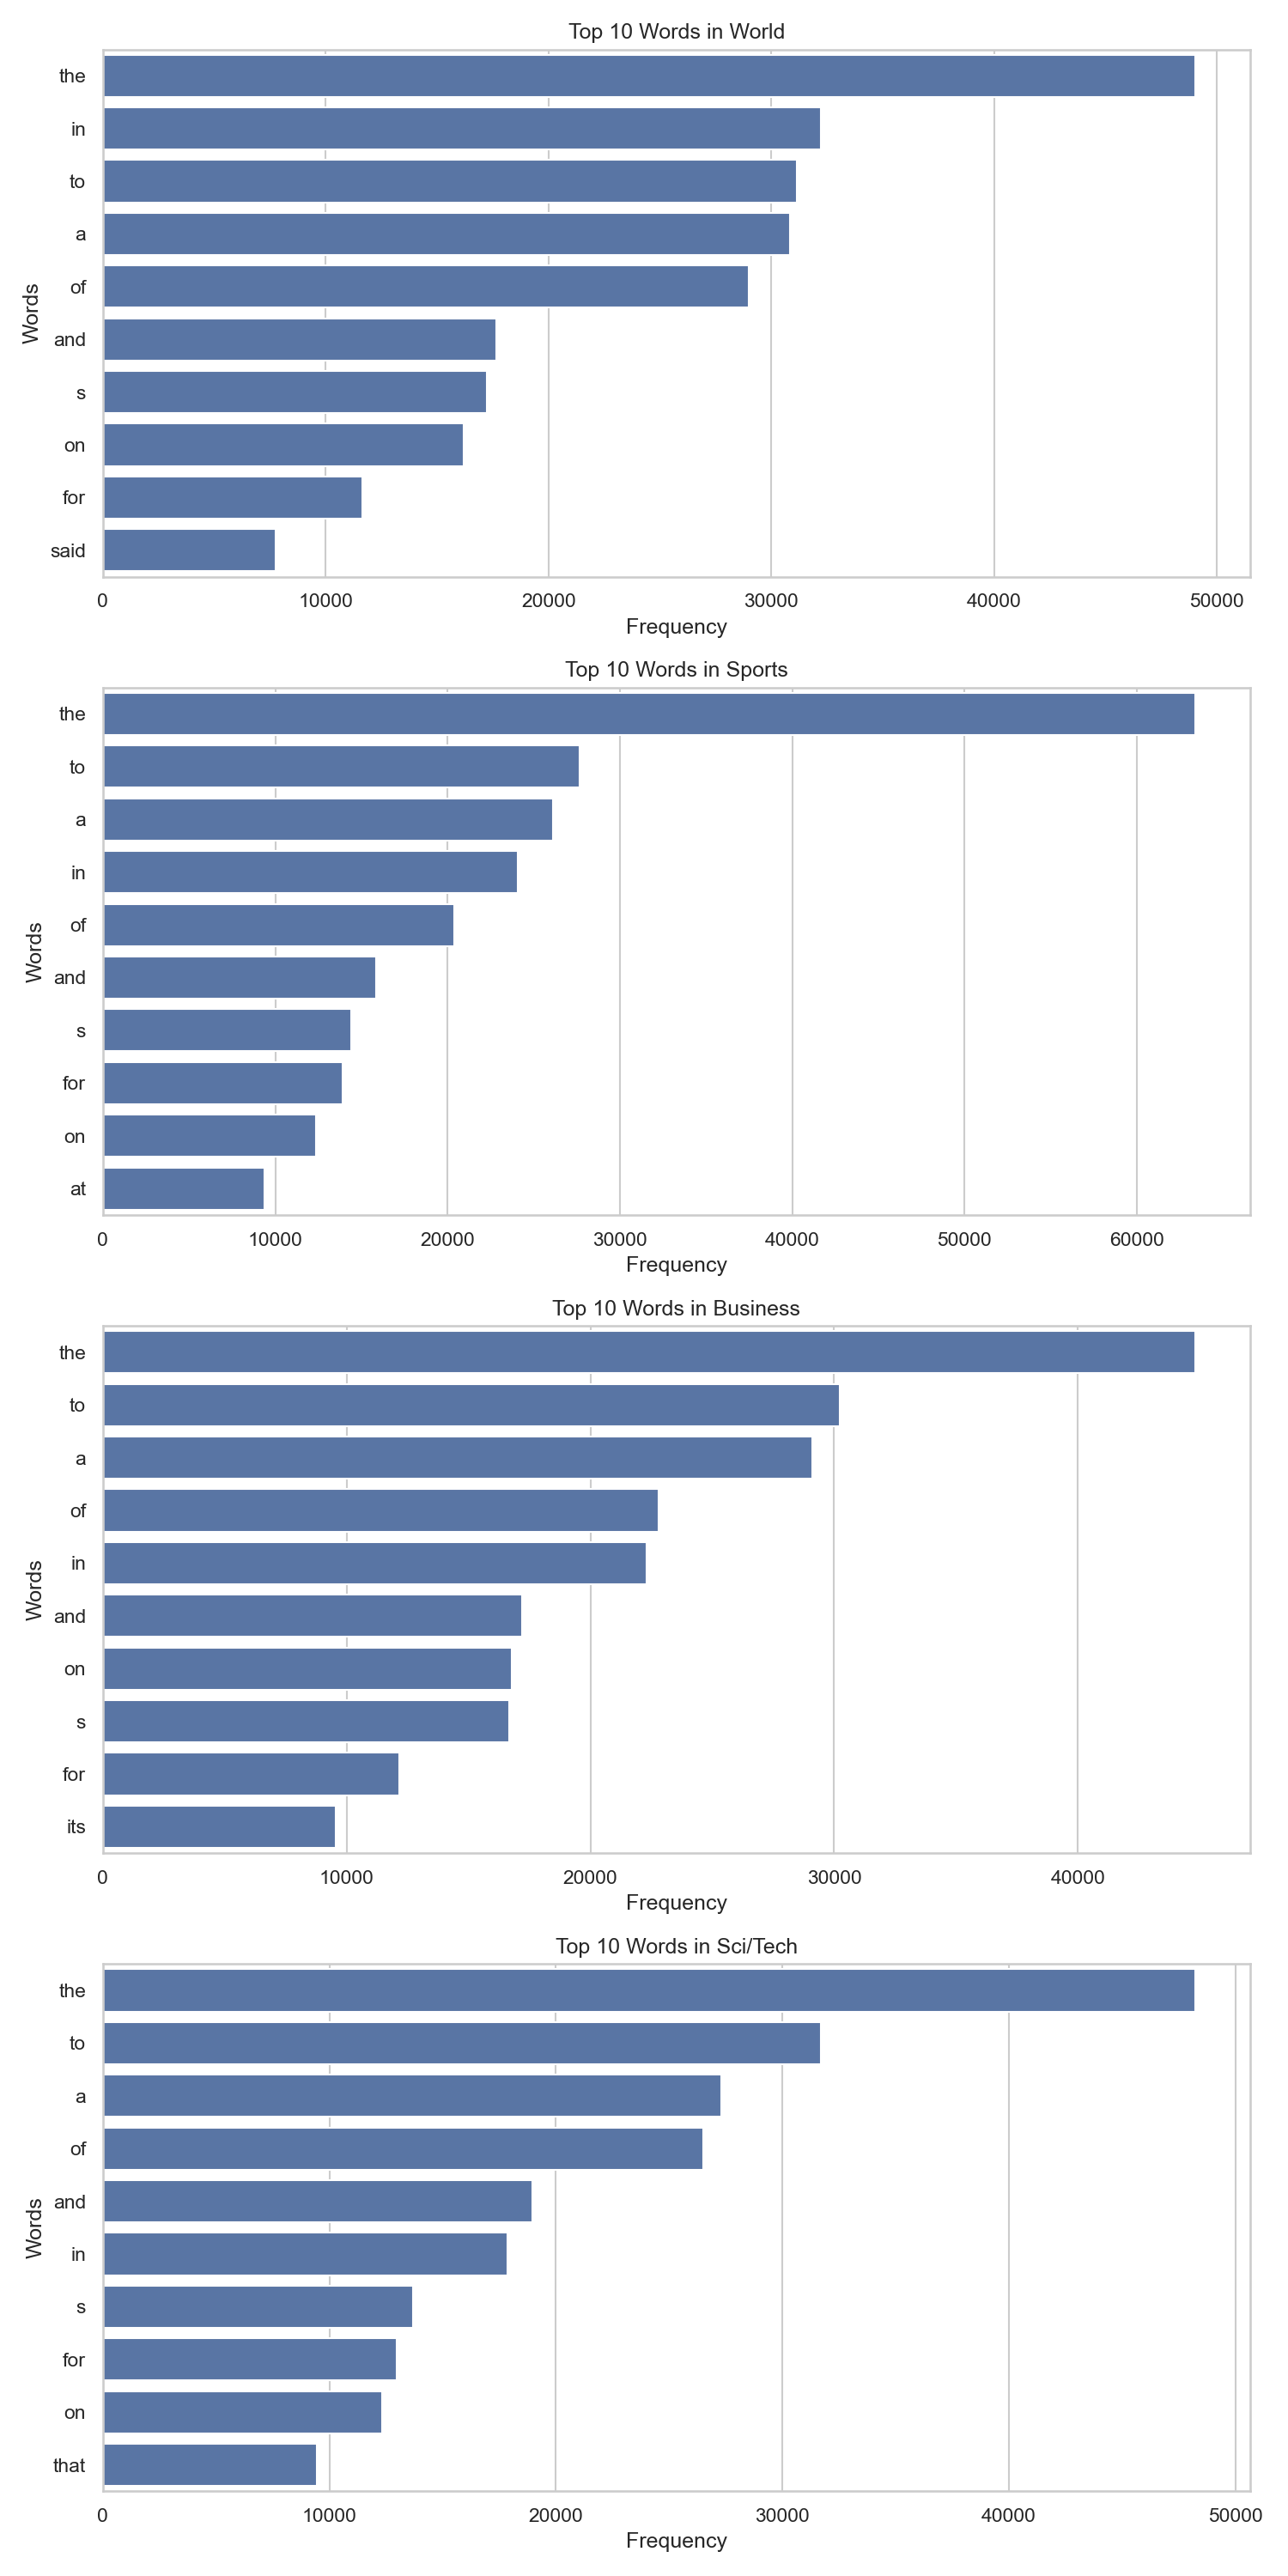
\includegraphics[width=0.8\linewidth]{eda/word_frequency.png}
    \caption{Word Frequency Analysis across AG News}
\end{figure}

\section{Implemented Methodology}
\subsection{Traditional Pipeline}
\begin{itemize}[leftmargin=*]
    \item Preprocessing options: lowercasing, stopword removal, punctuation removal, number removal.
    \item TF-IDF configuration search over three candidates: \texttt{tfidf\_uni\_1k}, \texttt{tfidf\_uni\_bi\_3k}, and \texttt{tfidf\_uni\_bi\_5k}.
    \item Primary model-selection metric: F1-weighted.
    \item Trained models: Logistic Regression, SVM, Naive Bayes.
\end{itemize}

\subsection{Modern Embedding Extension}
\begin{itemize}[leftmargin=*]
    \item Embedding model: \texttt{sentence-transformers/all-MiniLM-L6-v2}.
    \item Benchmark scales: \texttt{5k\_2k} and \texttt{20k\_2k}.
    \item Embeddings and labels are exported to \texttt{.npy} artifacts.
\end{itemize}

\section{Results}
\subsection{Best TF-IDF Results (Full Data)}
\begin{table}[H]
\centering
\begin{tabular}{lcccc}
\toprule
Model & Accuracy & Precision (w) & Recall (w) & F1 (w) \\
\midrule
SVM & 0.9046 & 0.9044 & 0.9046 & 0.9044 \\
Logistic Regression & 0.9038 & 0.9036 & 0.9038 & 0.9036 \\
Naive Bayes & 0.8871 & 0.8866 & 0.8871 & 0.8867 \\
\bottomrule
\end{tabular}
\caption{TF-IDF model comparison.}
\end{table}

\begin{figure}[H]
    \centering
    \begin{subfigure}[b]{0.32\textwidth}
        \centering
        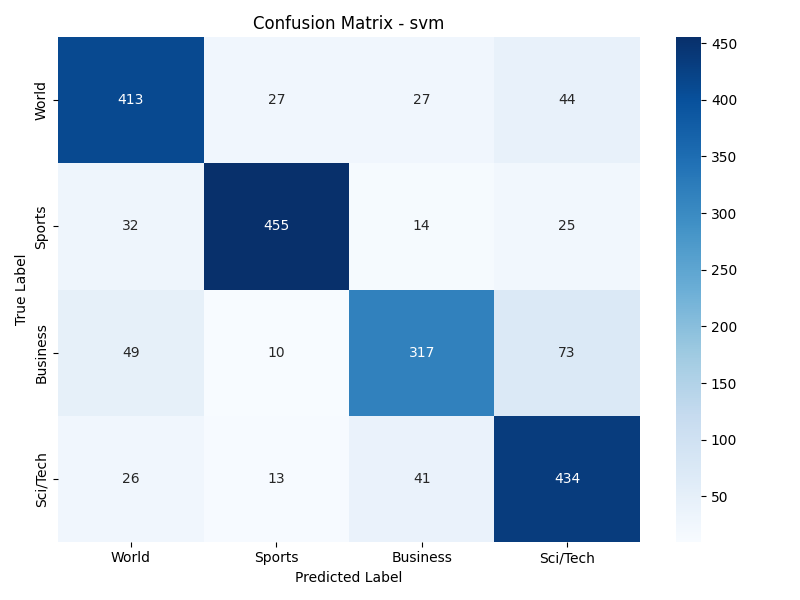
\includegraphics[width=\textwidth]{figures/cm_svm.png}
        \caption{SVM}
    \end{subfigure}
    \hfill
    \begin{subfigure}[b]{0.32\textwidth}
        \centering
        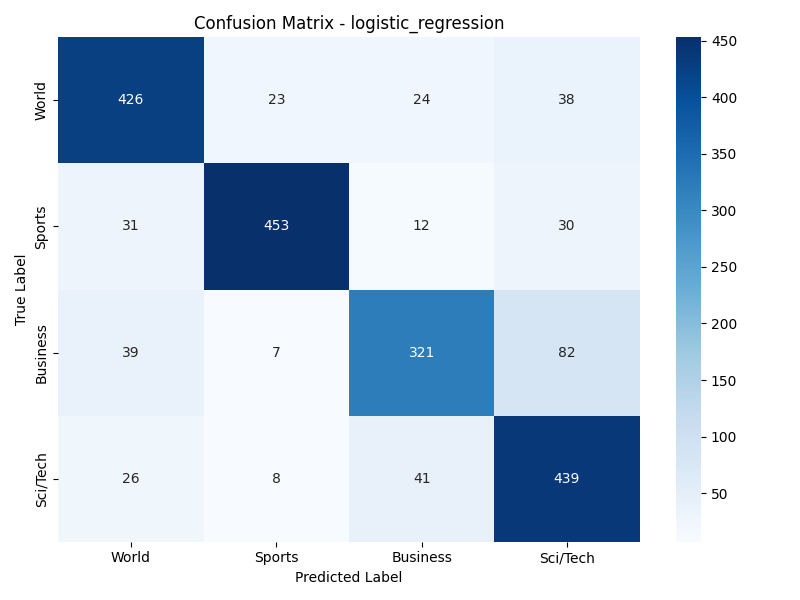
\includegraphics[width=\textwidth]{figures/cm_logistic_regression.png}
        \caption{LogReg}
    \end{subfigure}
    \hfill
    \begin{subfigure}[b]{0.32\textwidth}
        \centering
        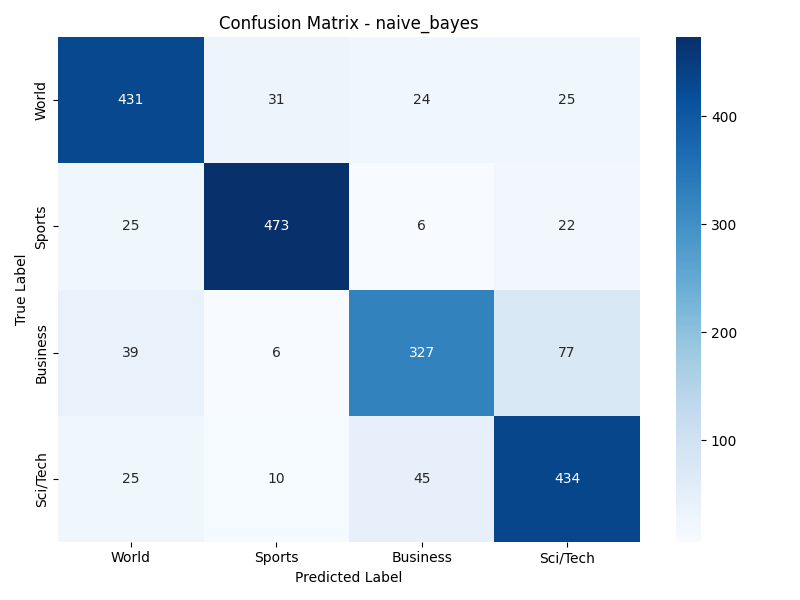
\includegraphics[width=\textwidth]{figures/cm_naive_bayes.png}
        \caption{Naive Bayes}
    \end{subfigure}
    \caption{Confusion Matrices for Traditional Models}
\end{figure}

\subsection{SBERT Benchmark Results}
\begin{table}[H]
\centering
\begin{tabular}{lccccc}
\toprule
Scale & Best Model & Accuracy & Precision (w) & Recall (w) & F1 (w) \\
\midrule
5k\_2k & Logistic Regression & 0.8740 & 0.8734 & 0.8740 & 0.8736 \\
20k\_2k & SVM & 0.8955 & 0.8958 & 0.8955 & 0.8954 \\
\bottomrule
\end{tabular}
\caption{Best embedding model per scale.}
\end{table}

\subsection{Feature-Family Comparison}
\begin{figure}[H]
    \centering
    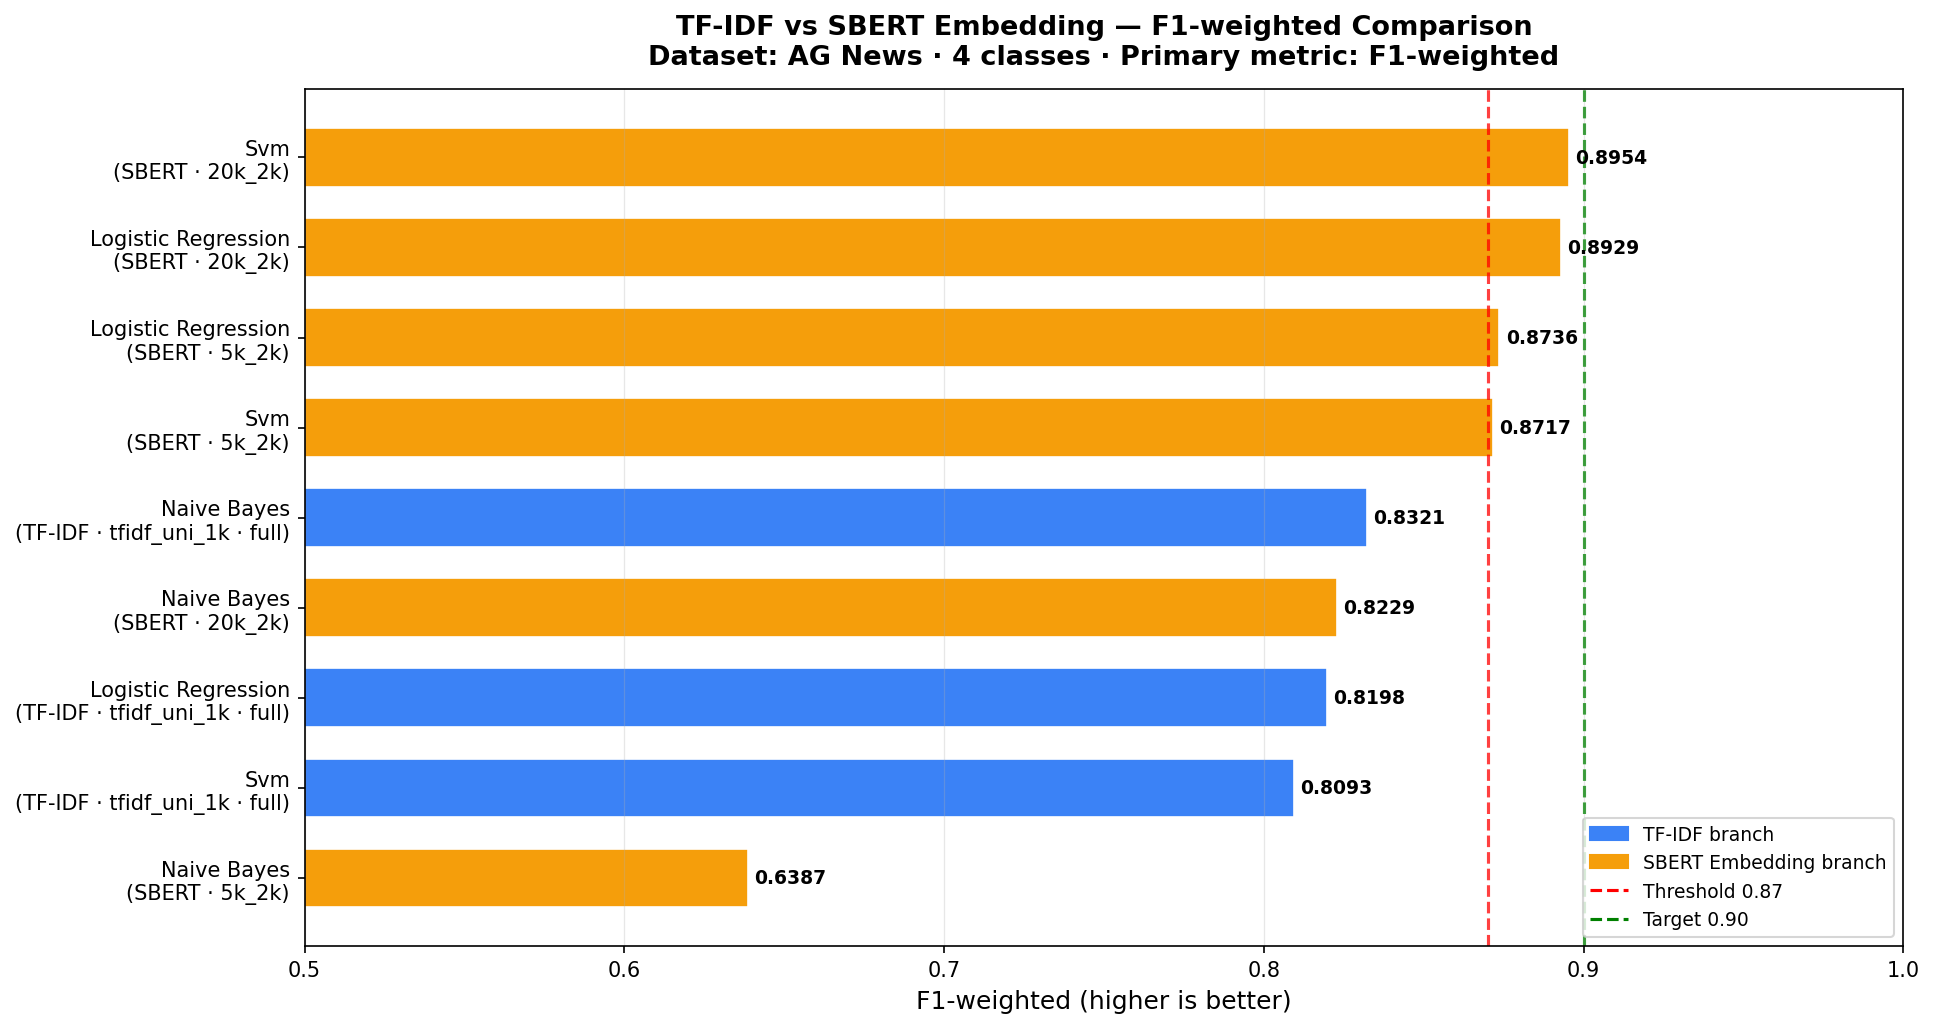
\includegraphics[width=0.85\linewidth]{figures/comparison_tfidf_vs_embedding.png}
    \caption{Performance Comparison: TF-IDF vs SBERT Embedding}
\end{figure}

The final comparison shows that the best TF-IDF model (SVM with F1 = 0.9044) outperforms the best SBERT embedding model (SVM at 20k scale with F1 = 0.8954). TF-IDF is significantly faster to train and extract, while maintaining highly interpretable sparse features. Therefore, TF-IDF + SVM is the primary recommendation.

\section{Error Analysis}
An error analysis was performed on the best TF-IDF model (SVM) to understand the distribution of misclassifications. Out of 7,600 test samples, the SVM model made 381 errors.

The top 3 most common confusion pairs are:
\begin{enumerate}
    \item \textbf{True: Business $\rightarrow$ Predicted: Sci/Tech} (73 occurrences)
    \item \textbf{True: Business $\rightarrow$ Predicted: World} (49 occurrences)
    \item \textbf{True: World $\rightarrow$ Predicted: Sci/Tech} (44 occurrences)
\end{enumerate}
This indicates a semantic overlap between Business/Technology news and Business/World news, which is common in articles discussing international tech corporations or global markets.

\section{Team Contributions}
\begin{table}[H]
\centering
\begin{tabularx}{\linewidth}{l c l X c}
\toprule
Member & ID & Email & Main Contribution & \% \\
\midrule
Tran Hoang Vy Khang & 2352502 & 2352502@hcmut.edu.vn & Embeddings, workflow, integration & 30 \\
Le Tan Minh Khoa & 2352563 & 2352563@hcmut.edu.vn & Text cleaning and TF-IDF & 20 \\
Tao Nguyen Quang Khang & 2352499 & 2352499@hcmut.edu.vn & ML training and evaluation & 20 \\
Tran Gia Huy & 2252264 & 2252264@hcmut.edu.vn & Pipeline and config architecture & 15 \\
Vo Le Hai Dang & 2352257 & 2352257@hcmut.edu.vn & Data loading and EDA analysis & 15 \\
\bottomrule
\end{tabularx}
\caption{Detailed contribution table with student emails.}
\end{table}

\end{document}
